\subsection{CLIP-GS}

\begin{Frame}{Key Insight}
	\begin{figure}[htbp]
		\centering
		\begin{annotatedFigureEnv}
			{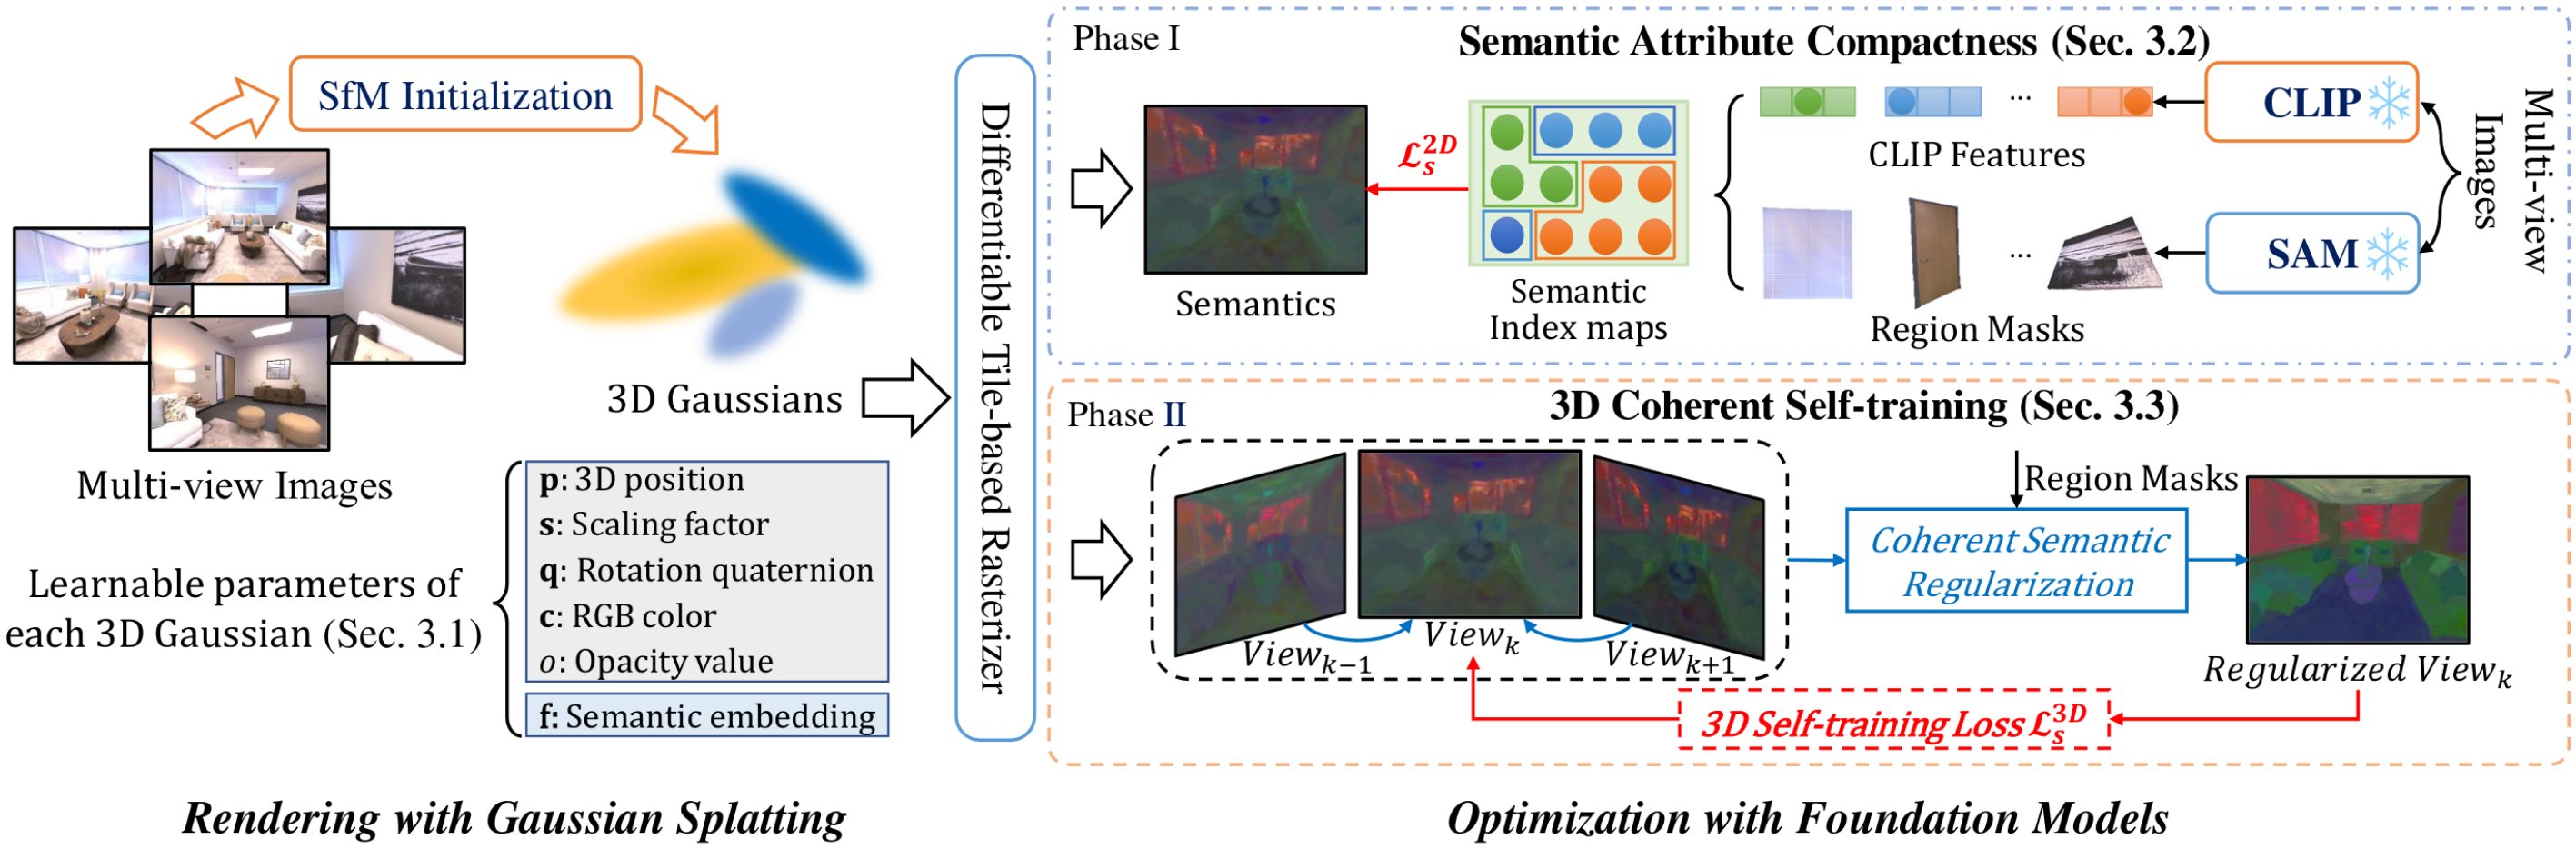
\includegraphics[width=0.7\linewidth]{clip-gs-overview.png}}
			\only<2|handout:1>{\annotatedFigure{0.41,0.57}{1,0.99}{1}{0.41,1.03}}
			\only<3|handout:1>{\annotatedFigure{0.41,0.10}{1,0.55}{2}{0.41,0.58}}
		\end{annotatedFigureEnv}
		\caption{Overview of CLIP-GS}
	\end{figure}
	\begin{enumerate}
		\setlength{\itemsep}{1.5ex}
		\item<2-> \alert<2>{Efficiency:} unify semantic features within an object by leveraging \alert<2>{SAM}.
		\item<3-> \alert<3>{Consistency:} supervise consecutive frames by \alert<3>{video segmentation}.
	\end{enumerate}
	\blfootnote{\href{http://arxiv.org/abs/2404.14249}{(arXiv 04/2024) CLIP-GS: CLIP-informed Gaussian Splatting for Real-time and View-consistent 3D Semantic Understanding}}
\end{Frame}

% \begin{frame}{Methodology: SAC \romannum{1} \hspace{0pt plus 1filll} \small Related Work \(\triangleright\) Semantic 3DGS \(\triangleright\) CLIP-GS}
% 	\colorlet{0_color}{cyan}
% 	\colorlet{0_color_marknode}{0_color!50}
% 	\colorlet{0_color_annotate}{0_color}
% 	\colorlet{1_color}{green}
% 	\colorlet{1_color_marknode}{1_color!50}
% 	\colorlet{1_color_annotate}{1_color}
% 	\vspace*{\fill}
% 	Unify semantic features from CLIP by leveraging SAM,
% 	\begin{figure}[htbp]
% 		\centering
% 		\begin{equation}
% 			\left\{\mathbf{F}^{(0)}, \mathbf{F}^{(1)}, \cdots, \tikzmarknode{index_label}{\colorbox{0_color_marknode}{\(\mathbf{F}^{(m)}\)}}, \cdots, \mathbf{F}^{(M)}\right\}=\operatorname{SAM}\left(\tikzmarknode{semantic-feature-image-clipgs}{\colorbox{1_color_marknode}{\(\mathbf{F}\)}}\right),
% 		\end{equation}
% 		\begin{tikzpicture}[overlay,remember picture,>=stealth,nodes={align=left,inner ysep=1pt},<-]
% 			\path (index_label.north) ++ (0em,0.5em) node[anchor=south east,color=0_color_annotate] (index_label_annotate) { \scriptsize \makecell[l]{\(:=\left\{(i,j,\mathbf{f}^{(m)}) \vert \operatorname{label}(i,j)=m\right\}\)}};
% 			\draw [color=0_color_annotate] (index_label.north) |- (index_label_annotate.south west);
% 			\path (semantic-feature-image-clipgs.north) ++ (0em,0.5em) node[anchor=south west,color=1_color_annotate] (semantic-feature-image-clipgs_annotate) { \scriptsize \makecell[l]{\(\in \mathbb{R}^{H\times W\times D}\)} };
% 			\draw [color=1_color_annotate] (semantic-feature-image-clipgs.north) |- (semantic-feature-image-clipgs_annotate.south east);
% 		\end{tikzpicture}
% 	\end{figure}
% 	where the representative semantic feature is a weighted average,
% 	\begin{equation}
% 		\mathbf{f}^{(m)} := \frac{1}{m} \sum_{(i,\,j)}^{\mathbf{F}^{(m)}} w^{(i,\,j)}\cdot\operatorname{CLIP}\left(\mathbf{c}^{(i,\,j)}\right).
% 	\end{equation}
% 	\vspace*{\fill}
% 	\blfootnote{\href{http://arxiv.org/abs/2404.14249}{[arXiv 04/2024] {CLIP}-{GS}: {CLIP}-informed Gaussian Splatting for Real-time and View-consistent 3D Semantic Understanding}}
% \end{frame}
% 
% \begin{frame}{Methodology: SAC \romannum{2} \hspace{0pt plus 1filll} \small Related Work \(\triangleright\) Semantic 3DGS \(\triangleright\) CLIP-GS}
% 	\colorlet{0_color}{cyan}
% 	\colorlet{0_color_marknode}{0_color!50}
% 	\colorlet{0_color_annotate}{0_color}
% 	\colorlet{1_color}{green}
% 	\colorlet{1_color_marknode}{1_color!50}
% 	\colorlet{1_color_annotate}{1_color}
% 	\vspace*{\fill}
% 	Therefore, we have the semantic index map, i.e. a look-up table,
% 	\begin{figure}[htbp]
% 		\vspace*{-2em}
% 		\centering
% 		\begin{equation}
% 			\mathcal{M}: \tikzmarknode{semantic-index-map}{\colorbox{0_color_marknode}{\(\mathbb{N}_{+}^{H \times W}\)}} \mapsto \tikzmarknode{representative-semantic-feature}{\colorbox{1_color_marknode}{\(\mathbb{R}^{D}\)}}.
% 		\end{equation}
% 		\begin{tikzpicture}[overlay,remember picture,>=stealth,nodes={align=left,inner ysep=1pt},<-]
% 			\path (semantic-index-map.south) ++ (0em,-1em) node[anchor=north east,color=0_color_marknode] (semantic-index-map_annotate) { \scriptsize \makecell[l]{semantic index map} };
% 			\draw [color=0_color_marknode] (semantic-index-map.south) |- (semantic-index-map_annotate.south west);
% 			\path (representative-semantic-feature.south) ++ (0em,-1em) node[anchor=north west,color=1_color_marknode] (representative-semantic-feature_annotate) { \scriptsize \makecell[l]{representative semantic feature} };
% 			\draw [color=1_color_marknode] (representative-semantic-feature.south) |- (representative-semantic-feature_annotate.south east);
% 		\end{tikzpicture}
% 	\end{figure}
% 	\vspace*{\fill}
% 	\par We learn the semantic index map, instead of semantic features, by leveraging
% 	\vspace*{1.5ex}
% 	\begin{enumerate}
% 		\setlength{\itemsep}{1.5ex}
% 		\item super low-dimensional Gaussian-wise embeddings, e.g. \(\dim= 3\);
% 		\item a classification head.
% 	\end{enumerate}
% 	\vspace*{\fill}
% \end{frame}
% 
% % \begin{frame}{Methodology: 3DCS \hspace{0pt plus 1filll} \small Related Work \(\triangleright\) Semantic 3DGS \(\triangleright\) CLIP-GS}
% % 	\vspace*{\fill}
% % 	TODO
% % 	% \par Use a pre-trained video tracker to associate SAM masks across consecutive frames.
% % 	\vspace*{\fill}
% % \end{frame}
% % 
% % \begin{frame}{Methodology: Training \hspace{0pt plus 1filll} \small Related Work \(\triangleright\) Semantic 3DGS \(\triangleright\) CLIP-GS}
% % 	\vspace*{\fill}
% % 	TODO
% % 	\vspace*{\fill}
% % \end{frame}
% 
% \begin{frame}{Limitations \hspace{0pt plus 1filll} \small Related Work \(\triangleright\) Semantic 3DGS \(\triangleright\) CLIP-GS}
% 	\vspace*{\fill}
% 	\begin{enumerate}
% 		\setlength{\itemsep}{3em}
% 		\item SAM is not perfect.
% 		      \vspace*{1.5ex}
% 		      \begin{itemize}
% 			      \setlength{\itemsep}{1.5ex}
% 			      \item What happens if masks are inaccurate?
% 			      \item How can we choose an adequate granularity adaptively?
% 		      \end{itemize}
% 		\item 3D consistency is maintained locally, not globally.
% 		      \vspace*{1.5ex}
% 		      \begin{itemize}
% 			      \setlength{\itemsep}{1.5ex}
% 			      \item A 2D video segmentation model can only supervise consecutive frames.
% 		      \end{itemize}
% 	\end{enumerate}
% 	\vspace*{\fill}
% \end{frame}
% 
% \subsubsection*{RT-GS2}
% \begin{frame}{Overview\hspace{0pt plus 1filll} \small Related Work \(\triangleright\) Semantic 3DGS \(\triangleright\) RT-GS2}
% 	\vspace*{\fill}
% 	\begin{block}{Key Insight}
% 		\par Learn view-indenpendent semantic features by self-supervision to enhance 3D consistency.
% 	\end{block}
% 	\vspace*{\fill}
% 	\begin{figure}[htbp]
% 		\begin{minipage}[c]{0.35\linewidth}
% 			\centering
% 			\includegraphics[width=\linewidth]{rt-gs2-overview.png}
% 		\end{minipage}
% 		\vspace*{\fill}
% 		\begin{minipage}[c]{0.60\linewidth}
% 			\begin{enumerate}
% 				\setlength{\itemsep}{3ex}
% 				\item \textbf{V}iew-\textbf{I}ndenpendent \textbf{F}eature:\\[1.5ex]
% 				      leverage an auto-encoder for contrastive learning across multi-views.
% 				\item \textbf{V}iew-\textbf{I}ndenpendent \& \textbf{V}iew-\textbf{D}enpendent \textbf{F}eature \textbf{F}usion
% 			\end{enumerate}
% 		\end{minipage}
% 	\end{figure}
% 	\vspace*{\fill}
% \end{frame}

% \subsubsection*{CoSSegGaussians}
% \begin{frame}{Overview \hspace{0pt plus 1filll} \small Related Work \(\triangleright\) Semantic 3DGS \(\triangleright\) CoSSegGaussians}
% 	\vspace*{\fill}
% 	\begin{block}{Key Insight}
% 		\par
% 	\end{block}
% 	\vspace*{\fill}
% 	\begin{figure}[htbp]
% 		\begin{minipage}[c]{0.35\linewidth}
% 			\centering
% 			\includegraphics[width=\linewidth]{cosseggaussians-overview.png}
% 		\end{minipage}
% 		\hspace{\fill}
% 		\begin{minipage}[c]{0.60\linewidth}
% 			\centering
% 			\begin{enumerate}
% 				\setlength{\itemsep}{1.5ex}
% 				\item Hello
% 			\end{enumerate}
% 		\end{minipage}
% 	\end{figure}
% \end{frame}
% 
% 
% \subsubsection*{Fast-LGS}
% \begin{frame}{Overview \hspace{0pt plus 1filll} \small Related Work \(\triangleright\) Semantic 3DGS \(\triangleright\) Fast-LGS}
% 	\vspace*{\fill}
% 	TODO
% 	\vspace*{\fill}
% \end{frame}
% \begin{frame}{Methodology: \hspace{0pt plus 1filll} \small Related Work \(\triangleright\) Semantic 3DGS \(\triangleright\) Fast-LGS}
% 	\vspace*{\fill}
% 	\begin{block}{Motivation}
% 		A vanilla integration of Gaussian-wise CLIP features,
% 		\begin{enumerate}
% 			\setlength{\itemsep}{1.5ex}
% 			\item computation \& memory inefficiency
% 			\item inconsistency and inaccuracy
% 		\end{enumerate}
% 		MLP-based compression
% 	\end{block}
% 	\vspace*{\fill}
% \end{frame}
